% !TEX TS-program = pdflatex
% !TEX encoding = UTF-8 Unicode

% This is a simple template for a LaTeX document using the "article" class.
% See "book", "report", "letter" for other types of document.

\documentclass[11pt]{article} % use larger type; default would be 10pt

%\usepackage[utf8]{inputenc} % set input encoding (not needed with XeLaTeX)


%%% Examples of Article customizations
% These packages are optional, depending whether you want the features they provide.
% See the LaTeX Companion or other references for full information.

%%% PAGE DIMENSIONS
\usepackage{geometry} % to change the page dimensions
\geometry{a4paper} % or letterpaper (US) ocher a5paper or....
\geometry{margin=1in} % for example, change the margins to 2 inches all round
% \geometry{landscape} % set up the page for landscape
%   read geometry.pdf for detailed page layout information

\usepackage{graphicx} 
% \usepackage[parfill]{parskip} % Activate to begin paragraphs with an empty line rather than an indent

%%% PACKAGES
%\usepackage{booktabs} % for much better looking tables
\usepackage{array} % for better arrays (eg matrices) in maths
%\usepackage{paralist} % very flexible & customisable lists (eg. enumerate/itemize, etc.)
\usepackage{verbatim} % adds environment for commenting out blocks of text & for better verbatim
%\usepackage{subfig} % make it possible to include more than one captioned figure/table in a single float
% These packages are all incorporated in the memoir class to one degree or another...

%%% HEADERS & FOOTERS
\usepackage{fancyhdr} % This should be set AFTER setting up the page geometry
\pagestyle{fancy} % options: empty , plain , fancy
\renewcommand{\headrulewidth}{0pt} % customise the layout...
\lhead{}\chead{}\rhead{}
\lfoot{}\cfoot{\thepage}\rfoot{}

%%% SECTION TITLE APPEARANCE
%\usepackage{sectsty}
%\allsectionsfont{\sffamily\mdseries\upshape} % (See the fntguide.pdf for font help)
% (This matches ConTeXt defaults)

%%% ToC (table of contents) APPEARANCE
%\usepackage[nottoc,notlof,notlot]{tocbibind} % Put the bibliography in the ToC
%\usepackage[titles,subfigure]{tocloft} % Alter the style of the Table of Contents
%\renewcommand{\cftsecfont}{\rmfamily\mdseries\upshape}
%\renewcommand{\cftsecpagefont}{\rmfamily\mdseries\upshape} % No bold!

%\usepackage[T1]{fontenc}
\usepackage[latin9]{inputenc}
%\usepackage[active]{srcltx}
\usepackage{setspace}
\usepackage{lscape}
\doublespacing
\usepackage[english]{babel}

\begin{document}

\title{Approaches for Large Scale Metagenome Assembly}
\author{ACH, JMT, CTB}
\maketitle

\section{Introduction}  
Complex microbial communities operate at the heart of many crucial environmental, ecological, and biomedical processes.  From marine communities that conduct the majority of photosynthesis (Venter shotgun, Iversson), to soil communities that fix nitrogen (permafrost, susannah), to gut communities (Qin, enterotypes) that provide key nutrients, complex assemblages of microbes provide critical ecosystem functionality that underpins all of biology (National Research Council, 2007).  Given the challenges with studying these communities in situ (cite Handelsman?), we lack a fundamental understanding of the diversity and function of these communities, much less how they self-assemble, maintain themselves, and evolve through time.  
Advances in DNA sequencing technologies provide unprecedented access to the content and spatial structure of these communities through the extraction and sequencing of DNA sampled directly from the environment.  The predominant form of this shotgun metagenome data being currently being generated is short-read sequences from Illumina sequencing platforms (cite Qin, rumen, permafrost) which yields millions to billions of 100 to 150 basepair reads representing hundreds, thousands, or even millions of species.   In order to detect rare species in environmental samples, deep sequencing is necessary resulting in extremely large volumes of sequencing data, up to 50 Tbp for an individual gram of soil (cite Gans?).  

Both the read lengths and scale of sequencing data pose new challenges to traditional analysis approaches of sequencing data.  Short read lengths and their associated sequencing errors and biases have little biological signal and are noisy.  Analysis approaches, e.g. direct annotation against reference genomes, do not scale well for the volume of reads generated.  Homology-based approaches are further limiting since the majority of genes sequenced from metagenomes are not similar to known genes.  

\emph{De novo} assembly of raw sequencing data offers several advantages to metagenomic sequencing datasets.  It reduces the total number of sequences for analysis by identifying consensus sequences from overlapping reads.  In addition to reducing the volume of data, the assembled contigs are longer and provide gene order providing more information for analysis.  Importantly, \emph{de novo} assembly does not rely on the existence of reference genomes, allowing the discovery of novel elements.  

Current assembly tools do not scale to the volumes of metagenomic datasets being generated. Assembled metagenomes from the rumen, human gut, and permafrost soils required processing of only most abundant sequences.  Furthermore, traditional assemblers have been designed for the assembly of single genomes whose abundance distribution and diversity content are significantly different from the mixed populations of metagenomes.  Recently, many new metagenome-specific assemblers have been developed to address characteristics of mixed population assembly but these also are limited to sample diversity and volume.    

In this study, we present approaches to address the limitations of metagenomic de novo assembly.  We propose a two-step process for metagenomes prior to assembly.  First, we reduce the dataset volume by normalizing sequencing coverage and removing sequencing errors and biases.  Second, we partition reads based on biological connectivity.  The resulting partitions can be assembled in a variety of currently available assemblers with significant reductions in computational requirements.  For a human gut mock community sequencing dataset, we show that these approaches result in a relatively unchanged assembly.  We also demonstrate the application of these approaches on two of the largest published soil metagenomes which have previously been impossible to assemble. 

\section{Results}

\subsection{Case study:  Assembly of mock metagenome}

\subsubsection{Summary of approaches used on mock community dataset}

The HMP mock community dataset and its available draft reference genomes were used to evaluate our approaches towards data reduction and partitioning for \emph{de novo} metagenomic assembly.   Reads of the mock community dataset were initially digitally normalized to a coverage threshold of 20 (as previously described in Brown et al), reducing the total number of reads from 14 to 11 million.  Additionally, to remove possible sequencing artifacts associated with high coverage sequences (previously described in Howe et al), highly-abundant sequences (20-mers present at coverage greater than 50-fold) were filtered and the dataset was further normalized to a coverage of 10, resulting in a total of 9 million reads (Figure ~\ref{kmercoverage}).  Finally, the remaining reads were divided into disconnected sets of reads resulting in a total of 85,818 partitions containing greater than five reads (summarized in Table~\ref{datareduction}).

\subsubsection{Evaluation of data reduction through digital normalization and high abundance filtering}

In total, our approaches removed a total of 5.9 million reads (40\% of total reads) prior to assembly of the HMP mock dataset.  The effects of our approaches were evaluated by both the coverage of reference genomes in the remaining filtered reads and the ability to recover reference genomes through assembly.  Overall, the mock community dataset contained sequences from a total of 51 reference sequences of chromosomes and/or plasmids.  Based on the coverage of these references by unfiltered reads, we estimate that a total of 30 reference genomes were sequenced to a coverage of greater than 3-fold, ranging from 6-fold to 2,000-fold coverages (Table ~\ref{referencestats} and Figures ~\ref{coverage1} and ~\ref{coverage2}).  Comparing the basepair coverage of these reference genomes by both unfiltered and filtered datasets (considering only bases which had a coverage of greater than 1), we found that 91\% and 93\% of reference sequences were covered by unfiltered and filtered reads, respectively.  (Note to fix language here as unclear to Titus) 

Additionally, the coverage of reference genomes by the assembled contigs resulting from the unfiltered and filtered datasets were also compared, resulting in recoveries of 43\% and 44\% of references, respectively, using the Velvet assembler.  The unfiltered Velvet assembly contained 29,063 contigs and 38 million bp compared to the filtered Velvet assembly containing 30,082 contigs and 35 million bp (Table ~\ref{assemblystats}).  NOTE TO DISCUSS THESE NUMBERS, I.E. WHY IS SECOND NUMBER SMALLER BUT RECOVERS MORE.  Comparable recoveries of references from the unfiltered and filtered assemblies were obtained for the SOAPdenovo and Meta-IDBA assemblers.   Comparing the unfiltered and filtered Velvet assemblies, we found that the genomic content of both assemblies were similar, ~94\%, and furthermore, the normalized and partitioned assemblies were greater than 99\% identical to each other.  By reducing the number of reads and associated errors in the filtered dataset, we were able to reduce the time and memory requirements for de novo assembly.  Specifically, for the Velvet assembler, the data reduction took less than 4 hours, and the time and memory for assembly was reduced from 12 GB and 4 hours for the unfiltered dataset to 3 GB and less than an hour for the filtered dataset.   

After assembly, the abundances of assembled sequences can be estimated with the coverage of all original, unfiltered reads (Figure ~\ref{diginormreference}).   Likewise, the coverage of the available reference genomes can also be estimated, and abundances predicted from reference genomes and assemblies compared.  The abundances of assembled contigs for both unfiltered and filtered (digitally normalized) datasets were compared to the estimated abundances of reference genomes (Figure ~\ref{coveragecompare}).  Using a one-directional, paired t-test of squared deviations, we compared the differences between the estimated abundances of the unfiltered and filtered assembled contigs against those of the associated reference genomes.  As we expected the filtered assembly to have increased accuracy due to a reduction of errors, we used a one-sided t-test and found that abundance estimations from the filtered assembly were significantly closer to predicted abundances from reference genomes (p-value of 0.032).  

The ability to assemble sequences relies heavily on sequencing coverage.  Consequently, we examined the effects of sequencing coverage of the mock community dataset on the our resulting assembled contigs.  Overall, we found that above a sequencing coverage of 5, the large majority of reads which could be mapped to reference genomes were also assembled (Figure ~\ref{coveragehmp}).  Below this threshold, reads could be mapped to reference genomes but were less likely to be associated with assembled contigs in either the unfiltered or filtered assemblies.   

\subsubsection{Evaluation of partitioning reads based on connectivity}
We evaluated the effects of partitioning reads based on connectivity in the reduced dataset.  For the 9 million reads in the filtered dataset, we identified a total of 85,818 partitions containing a minimum of five reads and among these, 83,459 partitions contained reads originating from a single reference genome.  With the exception of one partition containing reads from 36 reference chromosomes and/or plasmids, all other partitions contained reads from less than nine genomes.  

We next examined the number of partitions associated with reads which could be aligned to reference genomes and found that, in general, reference genomes with high coverage had fewer partitions (Table ~\ref{referencestats}).  The average number of partitions in reference genomes with coverage greater than 25 was 112 partitions compared to an average of 2771 partitions for genomes with coverage below 25.  Notably, in cases where multiple partitions were associated with a reference genome, reads aligning to the same region of a reference genome were associated with the same partition (Figure ~\ref{partitionreference}).

To further assess the effects of filtering, we evaluated the recovery of an E. coli reference strain E24377A, NC\_009801.1 through the assembly of spiked strain E24377A reads into the mock community dataset.  This ``spiked" mock community dataset was processed identically to the original mock dataset, resulting in similar amounts of data reduction after digital normalization and partitioning (Table ~\ref{referencestats}).  Among the 81,154 partitioned sets of reads, we identified that 78,574 partitions contained reads from only one genome, either an isolate reference genome or the spiked E. coli genome.  Overall, a total of 424 partitions contained reads from the spiked E. coli genome, among these 201 partitions contained emph{only} spiked reads (Figure ~\ref{ecolimap}).  The assembly of these 424 partitions resulted in contigs which when aligned against the E. coli strain E24377A genome overlapped 99.5\% (4957067 of 4979619 bp) of the original reference.

We performed a similar analysis on five closely-related E. coli strains.  Simulated sequencing reads were generated from completed genomes and added to the mock community dataset.  Partitioning the normalized and filtered ``mix-spiked" mock community dataset resulted in 81,425 partitions, of which 78,905 partitions contained reads originating from a single genome and 1,154 partitions contained reads associated with multiple genomes.  The remaining 1,366 partitions contained reads which were not aligned to any reference genomes.  Among the partitions which contained reads associated with a single genome, 658 partitions contained reads originating from a spiked E. coli strain.  In partitions containing greater than one genome, 224 partitions contained reads from a spiked E. coli strain and either another spiked strain or from the mock community dataset (Figure ~\ref{ecolimap}).  The partitions containing any reads originating from the spiked E. coli strains were identified and assembled independently.  Among the resulting 6,076 contigs, all but three contigs could be identified as originating from a spiked E. coli genome (e.g., top blast hit).  The remaining three contigs were greater than 99\% similar to HMP mock reference genomes (NC\_000915.1, NC\_003112.2, and NC\_009614.1) .  The E. Coli associated contigs were aligned against the spiked reference genomes, recovering greater than 98\% of each of the five genomes.  Many of these contigs were associated with reads from multiple genomes (Figure ~\ref{fractionassembled}), 3,075 contigs (51\%) contained reads which were mapped from more than one spiked genome.  This result is comparable to the fraction of contigs which are associated with multiple genomes when the same dataset is assembled without our approaches.  The unfiltered assembly of this dataset resulted in 4,702 contigs associated with the ``spiked reads", of which 66\% contained reads originating from more than one spiked genome.

\subsection{Characteristics of soil metagenomes}

We extended our approaches for the de novo assembly of two soil metagenomes.  Previously, the assembly of the Iowa corn and prairie datasets containing 1.8 billion and 3.3 billion reads, respectively, were impossible in 500 GB of memory.   A 75 million reads subset of the Iowa corn dataset alone required 110 GB of memory (Figure ~\ref{memory}).  Applying the same filtering approaches as applied to the HMP mock dataset, we reduced the Iowa corn and prairie datasets to 1.4 million and 2.2 million reads, respectively, and after partitioning, a total of 1.0 million and 1.7 million reads remained, respectively.  

The Iowa corn and prairies were sampled at significantly lower sequencing coverages than the HMP mock community dataset.  Whereas has the HMP dataset had only 33\% of its k-mers (k=20) present less than ten-times in the dataset, the Iowa corn and prairie datasets contained 53\% and 43\%, respectively, of all k-mers with less than ten-fold coverage.  The large majority of k-mers in the soil metagenomes are relatively low-coverage (Figure ~\ref{diginormcoverage}), and consequently, digital normalization did not remove as many reads in the soil metagenomes compared to the HMP dataset.

\subsubsection{Assembly of soil metagenomes}
	Based on the mock community dataset, we estimated that above a sequencing depth of 6, the large majority of sequences can be assembled (Figure ~\ref{coveragehmp}) for this human gut metagenome.  Given the greater diversity expected in the soil metagenomes, we normalized these datasets to a coverage threshold of 20.  Notably, low abundance reads would not be affected by this filtering approach.  After partitioning the filtered datasets, we identified a total 31,537,798 and 55,993,006 partitions (containing greater than five reads) in the corn and prairie datasets, respectively.  For practical assembly, partitions were grouped together such that groups contained partitions with similar numbers of reads and no group contained larger than 10 million reads.  Once partitioned, each group of reads could be assembled in less than 14 GB and 4 hours, enabling evaluation of multiple assemblers and various assembly parameters.
	The final Velvet assembly of the corn and prairie soil metagenomes resulted in a total of 1.9 million and 3.1 million contigs, respectively, and a total assembly length of 912 million bp and 1.5 billion bp, respectively.  To estimate abundance of assembled contigs and evaluate incorporation of reads, all quality-trimmed reads were aligned to Velvet assembled contigs (greater than 300 bp).  Overall, for the Iowa corn assembly, 8\% of single reads and 10\% of paired end reads mapped to the assembly.  Among the paired end reads, less than 0.5\% aligned disconcordantly.  Similar results were found for the Iowa prairie assembly with only 0.6\% paired ends aligned disconcordantly and slightly higher numbers of reads mapped with 10\% of single reads and 11\% paired end reads (Table ~\ref{mappings}).  The read coverages of assembled contigs within the soil metagenomes were estimated (Figure ~\ref{soilassemblycoverage}).  Overall, there is a positively skewed distribution of coverage of all contigs from both soil metagenomes, biased towards a coverage of less than ten-fold.  The Iowa corn and prairie assemblies contained 48\% and 31\% of total contigs with a median basepair coverage less than 10.  
	
\subsubsection{Content of soil metagenome assembly}
	To 


	Assembled contigs (greater than 300 bp) were annotated by the MG-RAST annotation pipeline.  In total, there were 2,046,698 and 3,410,388 predicted protein coding regions in Iowa corn and prairie assembled contigs, respectively, and among these, 848,422 and 1,169,437 features could be annotated by MG-RAST.   
	
	
	
	
	Using these annotations against SEED subsystems, the functional profile of assembled contigs was determined for Iowa corn and prairie metagenomes.  The 

HOUSEKEEPING GENES
NITROGEN CYCLE GENES
ABUNDANCES CORRELATED

\section{Discussion}

\subsection{Community sequencing has variable coverage motivating normalization} 

Reflective of diversity in the natural environment, all metagenomes consist of sequences originating from a mixture of genomes.  Similarly, the HMP mock community dataset used in this study originates from an uneven mixture of DNA extracted from 21 different bacterial strains.  Although the diversity represented by this mock community is extremely low compared to that of most environmental metagenomes, it represents a simplified dataset with the key advantage of the ability to evaluate analyses through the availability of source genomes.  Like metagenomes, this mock community dataset contains uneven sampling of various genomes, evidenced by reads present at a broad range of sequencing depths, from singletons to reads with abundances of greater than 255 and peaks of highly abundant reads at sequencing depths 8 and 21 (Figure ~\ref{kmercoverage}).   This read coverage is reflective of genomes present at high abundances which are readily sampled and result in reads present at high sequencing depth and conversely, under sampled genomes which are under sampled and result in reads with low sequencing depths.  

Using the mock community reference genomes, we could examine the sequencing depth of reads necessary for assembly.  For the mock community dataset, we found that among the reads which could be aligned to the reference genomes, if sequencing depth (basepair coverage) were greater than 6-fold, the large majority of reads could also be mapped to assembled contigs.  Below this threshold, reads were more unlikely to be present in assemblies, likely due to the lack of appropriately assembled sequences caused by low coverage and/or erroneous assembly.  With greater sequencing depth, the number of reads which could be mapped to both the reference genomes and the assembly did not change significantly, suggesting a sequencing coverage "sweet point" at which sufficient sequences are present with which to complete assembly and beyond which further sequencing is redundant.  

The sequences beyond this coverage threshold not only are redundant for the purpose of /emph de novo assembly but are also significant sources of error.  In previous studies of an Illumina E. Coli dataset, the removal of 90\% of normalized reads resulted in nearly an identical assembly of the E. Coli genome while removing over 50\% of the sequencing errors (Brown, diginorm paper).  Thus, the removal of redundant sequences from a dataset enables not only a more uniform coverage but also reduces the volume of sequences and errors prior to assembly.  To further remove errors from our dataset, we also targeted Illumina sequencing artifacts in metagenomes which have previously been shown to be correlated to high abundance sequences.  We removed high abundance sequences (20-mers greater than 50-fold coverage) from reads prior to assembly. 

For the HMP mock dataset, when we compared the assembly resulting from the filtered dataset to that of the unfiltered dataset, the content of both assemblies were very similar (94\%), and we were able to recover roughly the same fraction of reference genomes (~40\%).  For specific reference genomes, the fraction of assembled sequence recovered from the unfiltered and filtered assemblies were evaluated and also found to be similar (Figures ~\ref{coverage1} and ~\ref{coverage2}, blue and green lines).  Likewise, the fraction of references which could be mapped by unfiltered and filtered reads were comparable (Figures \ref{coverage1} and ~\ref{coverage2}, red and gray lines).  

For the very high coverage reference genomes, originating from three plasmids of \emph{Staphylococcus} epidermidis (NC\_005008.1, NC\_005007.1, and NC\_005003.1), filtered assemblies did not recover large portions of these genomes despite the comparable presence of filtered and unfiltered reads for two of the three plasmid genomes.  We found that shared regions among these genomes shared ~90\% identity over ~290 bp, suggesting the presence of repetitive elements among these genomes.  Such repetitive sequences would appear as high coverage elements during digital normalization and would be targetted for removal.  For the unfiltered assembly, where more of these regions were assembled, it is likely that the higher coverage of a larger span of repetitive regions enabled assembler heuristics to extend more assembly of these sequences.  

The observation of this result, though rare among the reference genomes, highlights a current shortcoming of our approach, and indeed for most short-read assembly approaches, related to repetitive regions and/or polymorphisms which should be considered in its application.  For the soil metagenomes described in this study, the data reduction made possible by our methods may cause the loss of information which may be useful for assembly, but we are at least able to complete assemblies which were previously not possible.  Evaluation with the HMP mock community dataset suggests that this information loss is minimal overall.  To further support the use of the reduced dataset assembly, we found that estimations of abundance of reference genomes based on the filtered assemblies were slightly more accurate compared to the unfiltered assembly of the mock community dataset.

\subsection{Community sequencing is made up of connected genomes motivating partitioning}

A broad range of diversity must be represented in metagenomic assembly graphs. The continuous paths of short, overlapping sequences are used to determine read overlaps, i.e., reads originating from adjacent locations on a genome would be connected.   Two or more genomes which are thoroughly sequenced would be expected to be connected in a single assembly graph by conserved elements such as 16S rRNA genes.  For most metagenomes, however, the majority of constituent genomes are undersampled resulting in only fragments of connectivity.  Thus, metagenomic assembly graphs are expected to contain multiple, separate connected sets of reads or subgraphs representing sequences from different genomes or genomic fragments.  Our partitioning approach targets these subgraphs to divide large metagenomes into subsets which reflect the biological characteristics of the originating dataset.  

To enable partitioning of metagenomic datasets, we must first remove sequencing biases which cause artificial connectivity within metagenomic assembly graphs (Howe).  In the HMP mock community dataset, the removal of these sequences (combined with normalization) did not significantly alter the recovery of reference genomes through de novo assembly and enabled the division of the mock community dataset into thousands of disconnected partitions.  The resulting assembly of these partitions was nearly identical (>99\% similar) to the assembly of the reduced dataset.  The large majority of these partitions (>97\%) contained reads from a single reference genome, supporting our previous hypothesis that most connected subgraphs contain  distinct genomes.  In general, high coverage genomes contained fewer partitions because they were well-sampled with sequencing, and most reads could be connected together within the assembly graph.  Low coverage genomes contained more partitions as these assembly graphs were fragmented due to undersampling.  The same partition was associated with reads from fragmented regions (Figure ~\ref{partitionreference}) since these reads were connected within the assembly graph.  

We further demonstrate the success of our approaches to to recover sequences from one or more E. Coli strains computationally spiked into the mock community dataset.  For a spike of a single E. Coli strain, we identified the fraction of partitions containing associated reads and from these partitions alone could recover 99\% of the original genome (Figure ~\ref{ecolimap|}).  When closely related strains were spiked into the HMP dataset, we could recover the large majority of the genomic content of these strains but largely in chimeric contigs which contained reads from multiple reference genomes (Figure ~\ref{fractionassembled}).  However, this result is not unique to our approach as assemblies of the unfiltered dataset resulted in a slightly higher fraction of assembled contigs associated with multiple references. 

As discussed above, closely related sequences which result from either repetitive or inter-strain polymorphisms are a challenge to assemblers, and our approaches are not specifically designed to target such regions.  Interestingly, the partitions resulting from our approach (without digital normalization) could provide a subset of sequences which could be targeted for more sensitive assembly approaches for such regions (i.e. overlap-layout-consensus approaches).  

Most importantly, our partitioning approach subdivides our datasets into sets of reads which can be assembled in parallel, and consequently, with less computational resources.  For the soil metagenomes, we were able to assemble grouped partitions in less than a day and in under 14 GB of memory enabling the usage of multiple assembly parameters (e.g., k-length) and multiple assemblers (Velvet, soapdenovo, and meta-idba).

\subsection{What we gained from the soil assembly}

Results of fungene blasts
Titus's idea for phylogeny and diversity comparisons

\section{Conclusion}
CONCLUSION:  
THEME: PARTITIONING IS NOT ONLY AWESOME FOR ASSEMBLY BUT...

\section{Methods}

\subsection{Datasets}
In this study, we examined two large soil metagenomes generated from soils collected from Iowa corn and native prairie soils.  Sequencing was performed at the DOE Joint Genome Institute (Walnut Creek, CA).   Reads were quality trimmed at where Phred scores indicated a score of '2'.  The total quality-trimmed reads in the Iowa corn and prairie datasets were 1.8 million and 3.3 million, respectively.  We also include a human gut mock community dataset (combined from SRA SRX055381 and SRX055380).  For this mock community dataset, DNA from bacterial isolates originally recovered from within or on the human body was mixed together and sequenced.  The mock community dataset originally contained 14.5 million reads.  

To evaluate our approaches, we added simulated reads from either a single E. Coli (str. K-12 substr DH10B) or five E. coli strains (K-12 substr DH10B, E24377, O147:H7 str. EC4115, UMN026, SE15) into select metagenomes.  We computationally generated 100 bp reads from each reference genome to a coverage of 10x and with a 2\% error rate and subsequently randomly shuffled these reads with select datasets.

\subsection{Assembly Pipeline}
\subsubsection{Estimation of assembly requirements for soil metagenomes}
Subsets of the Iowa corn metagenome were assembled with the Velvet assembler (v1.2.07) with the following parameters:  velveth K=45, -short and velvetg -exp\_cov auto -cov\_cutoff auto, -scaffolding no.  The time and memory for each assembly was estimated up to a maximum of 150 hours and 100 GB.

\subsubsection{Digital normalization}
Digital normalization was previously describe in X.  For the mock community dataset, digital normalization was performed with the following parameters:  K=20, coverage=20, and bloom filter size = 1 GB x 4.  For Iowa corn metagenome, digital normalization parameters were as follows:  K=20, coverage=20, and bloom filter size = 48 GB x 4.  Similar parameters were used for the Iowa prairie metagenome, with the exception that the bloom filter size was 60 GB x 4.

\subsubsection{Removal of high abundance sequences}
To eliminate known sequencing artifacts in Illumina metagenomes (previously described in XXX), high abundance sequences (coverage greater than 50) were removed using the count-min-sketch datastructure used for digital normalization.  For the relatively high coverage mock community dataset, filtered reads were subsequently normalized to a coverage of 10 (K=20, bloom filter size = 1 GB x 4).  

\subsubsection{Partitioning and \emph{de novo} assembly of disconnected reads}
Normalized and filtered datasets were loaded into a probablistic representation of the assembly graph as previously described in Pell et al, and disconnected partitions of the resulting graph were separated.  Partitions containing less than 5 reads were discarded.  Each partition was subsequently assembled using the Velvet assembler with the same setting as describe as above, with the exception that K=35-59 and shortPaired setting was used for paired end reads.  The resulting contigs greater than 300 bp from multiple-K assemblies were dereplicated with CD-HIT (XXXX, 99\% similarity) and merged with Minimus2 (XXXX).  

\subsection{Comparing coverage of reference genomes by reads}
Reads in the HMP mock unfiltered and filtered datasets were mapped back to originating genomes using default settings in Bowtie2 (citation).  For cases where reads could be mapped back to multiple genomes, a single genome was randomly selected to be identified with each read.  Sequencing coverage was estimated for the whole genome as the median base pair coverage for all base pairs in reference genome.  

\subsection{Comparing assemblies}
Resulting assemblies (contigs greater than 300 bp) were compared using the total number of contigs, assembly length, and maximum contig size for each assembly.  Assemblies were also aligned to each another using blastn and the resulting coverage of each assembly was calculated.  In the case of the mock community, the resulting assemblies were also aligned to sequenced draft genomes of the original isolates and, if applicable, spiked reference genomes.

Abundance of assembled contigs and reference genomes were estimated by mapping raw reads with Bowtie (allowing up to 2 mismatches for a match).  The median base pair coverage was used to estimate abundances.  Associated assembled contigs (greater than 300 bp) from the unfiltered and filtered (digital normalized) assemblies were identified using a blastn alignment (requiring E-value cutoff of 1e-5).  Contigs were associated with reference genomes through an identical alignment approach.

\subsection{Identication of \emph{gyrB}, \emph{recA}, and \emph{rplB}}
Well-curated sequences from the Ribosomal Database Project's (RDP) Functional Gene Repository were used to build HMM profiles for \emph{gyrB}, \emph{recA}, and \emph{rplB}.  These models are available upon request from RDP.  The \emph{gyrB}, \emph{recA}, and \emph{rplB} HMM models contained 809, 353, and 277 amino acids, respectively.  Assembled contigs were translated in all six reading frames and searched against the HMM profiles using HMMER3 (v3.0).  Results were filtered with an E-value threshold of 1e-5.  The abundance of assembled contigs were previously calculated as described above and used to estimate total number of \emph{gyrB}, \emph{recA}, and \emph{rplB} genes within soil metagenomes.  We also evaluated our ability to identify these genes against the HMP mock reference dataset and found that in some cases, the genes were not identified for some isolates or multiple reading frames within a reference genome were found to contain the gene of interest.  We thus corrected calculated abundances of these genes based on our ability to identify the 22 HMP isolates using the described methods.  

\subsection{Figures and Tables}

\begin{landscape}
\begin{figure}[h!]
\center{\includegraphics[scale=0.8]{./figures/genome-coverage1.png}}
\caption{Coverage of reference genomes by unfiltered and filtered assembled contigs and unfiltered and filtered reads.}
\label{coverage1}
\end{figure}
\end{landscape}

\begin{landscape}
\begin{figure}[h!]
\center{\includegraphics[scale=0.8]{./figures/genome-coverage2.png}}
\caption{Coverage of reference genomes by unfiltered and filtered assembled contigs and unfiltered and filtered reads.}
\label{coverage2}
\end{figure}
\end{landscape}

\begin{landscape}
\begin{figure}[h!]
\center{\includegraphics[scale=0.5]{./figures/contig-lengths.pdf}}
\caption{Total number of contigs for unfiltered (bars with hashed lines) and filtered (solid bars) for top twenty references with most assembled contigs.  Red indicates contig lengths less than 500 bp, yellow indicates contig lengths between 500 bp and 3000 bp, and green indicates contig lengths greater than 5000 bp.}
\label{contig-lengths}
\end{figure}
\end{landscape}

\begin{figure}[h!]
\center{\includegraphics[width=\textwidth,height=\textheight,keepaspectratio]
{./figures/comparison-coverage.pdf}}
\caption{SUPPLEMENTAL:  Comparing the estimated coverage (median bp) of assembled unfiltered (red circles) and filtered (blue circles) contigs to coverage of reference genomes (median bp) based on mapped unfiltered reads.  The dotted-line indicates that abundance estimation from reference genomes and assembled contig is identical.}
\label{coveragecompare}
\end{figure}

\begin{figure}[h!]
\center{\includegraphics[width=\textwidth,height=\textheight,keepaspectratio]
{./figures/coverage.pdf}}
\caption{Number of basepairs with specified coverage for reads which map to reference genomes and unfiltered and filtered assembled contigs greater than 300 bp.}
\label{coveragehmp}
\end{figure}

\begin{figure}[h!]
\center{\includegraphics[width=\textwidth,height=\textheight,keepaspectratio]{./figures/ref_gi32470572.pdf}}
\caption{Alignment of reads (colored by originating partition) to reference genome NC\_00745901}
\label{diginormreference}
\end{figure}


\begin{figure}[h!]
\center{\includegraphics[width=\textwidth,height=\textheight,keepaspectratio]{./figures/NC_0074901.png}}
\caption{Alignment of reads (colored by originating partition) to reference genome NC\_00745901}
\label{partitionreference}
\end{figure}

\begin{figure}[h!]
\center{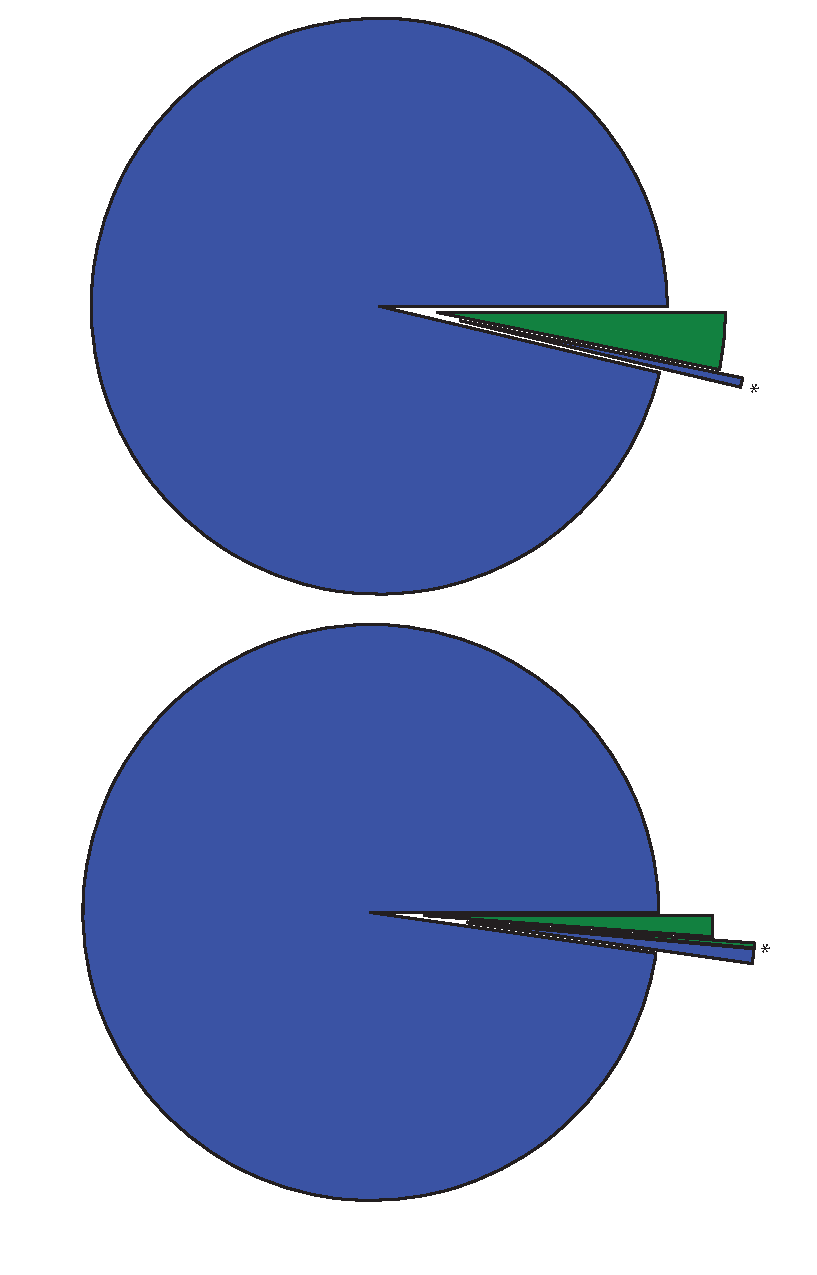
\includegraphics[width=\textwidth,height=\textheight,keepaspectratio]{./figures/ecolis-partitions.pdf}}
\caption{The fraction of partitions in spiked HMP datasets which contain single genomes (blue) and multiple genomes (green).  The section marked as * indicates partitions which contain spiked E. Coli reads which were subsequently assembled independently.  The top piechart is the single E. Coli spiked dataset and the bottom piechart is the multiple E. Coli spiked dataset.}
\label{ecolimap}
\end{figure}

\begin{figure}[h!]
\center{\includegraphics[width=\textwidth,height=\textheight,keepaspectratio]{./figures/ecoli-multi-genomes.png}}
\caption{The fraction of assembled contigs assembled from partitions containing spiked E. Coli reads associated with 0 to five of the E. Coli reference genomes.  The large majority of contigs contain reads associated with multiple genomes or to no genome.}
\label{fractionassembled}
\end{figure}

\begin{figure}[h!]
\center{\includegraphics[width=\textwidth,height=\textheight,keepaspectratio]{./figures/memory-requirements.png}}
\caption{Memory requirements to assemble subsets of Iowa corn soil metagenome}
\label{memory}
\end{figure}

\begin{figure}[h!]
\center{\includegraphics[width=\textwidth,height=\textheight,keepaspectratio]
{./figures/mockdiginormhist.pdf}}
\caption{K-mer coverage of HMP mock community dataset before and after filtering approaches.}
\label{kmercoverage}
\end{figure}

\begin{figure}[h!]
\center{\includegraphics[width=\textwidth,height=\textheight,keepaspectratio]
{./figures/soildiginorm.pdf}}
\caption{K-mer coverage of Iowa corn and prairie metagenomes before and after filtering approaches.}
\label{diginormcoverage}
\end{figure}

\begin{figure}[h!]
\center{\includegraphics[width=\textwidth,height=\textheight,keepaspectratio]
{./figures/assembly-coverage.pdf}}
\caption{Coverage (median basepair) distribution of assembled contigs from soil metagenomes.}
\label{soilassemblycoverage}
\end{figure}

\begin{landscape}
\begin{table}[h!]
\center{\includegraphics[scale=0.8]{./figures/data-reduction.pdf}}
\caption{The total number of reads in original, filtered, and partitioned datasets and the computational resources required for filtering and partitioning.}
\label{datareduction}
\end{table}
\end{landscape}

\begin{landscape}
\begin{table}[h!]
\center{\includegraphics[scale=1.0]{./figures/reference-genomes.pdf}}
\caption{Candidate for Suppl.:  HMP mock dataset reference genomes estimated sequencing depth (median bp coverage of reads), number of partitions, total length (bp), coverage of reference genomes by unfiltered reads, coverage of reference genomes by filtered reads, coverage of reference genomes by unfiltered assembled contigs, and coverage of reference genomes by filtered assembled contigs.}
\label{referencestats}
\end{table}
\end{landscape}

\begin{landscape}
\begin{table}
\center{\includegraphics[scale=1.2]{./figures/assembly-stats.pdf}}
\caption{Assembly comparisons of unfiltered and filtered or filtered/partitioned datasets.  Assembly content similarity is based on the fraction of alignment of assemblies and similarly, the coverage of reference genomes is based on the alignment of assembled contigs to reference genomes.  Assembly summary statistics are also shown for multiple assemblers.}
\label{assemblystats}
\end{table}
\end{landscape}

\begin{landscape}
\begin{table}
\center{\includegraphics[scale=1.2]{./figures/mapping-summary-gpgc.pdf}}
\caption{Fraction of single-end (SE) and paired-end (PE) reads mapped to Iowa corn and prairie assemblies.}
\label{mappings}
\end{table}
\end{landscape}



\end{document}